\documentclass[presentation]{beamer}
\usepackage{../oop-slides-pianini}
\setbeamertemplate{bibliography item}[text]
\newcommand{\lessonnr}[0]{10}
\title[OOP10 -- DVCS Workflow]{10\\ Strategie di uso efficace dei \\ Decentralized Version Control Systems}

\begin{document}

\frame[label=coverpage]{\titlepage}

%====================
%Outline
%====================
\begin{frame}<beamer>
 	\frametitle{Outline}
 	\tableofcontents[]
\end{frame}

\section{Preparazione al laboratorio}

\begin{frame}{Preparazione dell'ambiente di lavoro}
	\begin{enumerate}
		\item Clonare il repository degli esercizi
		\begin{itemize}
			\item \url{https://bitbucket.org/danysk/courses-2017-oop-lab-09}
			\begin{itemize}
				\item Opzionalmente, si fork-i il repository
			\end{itemize}
			\item Si copi la URI con cui effettuare il clone dall'interfaccia web di Bitbucket
		\end{itemize}
		\item Importare il repository in Eclipse come progetto Java
		\begin{enumerate}
			\item File
			\item Import
			\item General
			\item Existing project into workspace
			\item Si selezioni la cartella del progetto
			\item Si confermi l'import
		\end{enumerate}
		\item Configurare correttamente Eclipse, abilitare e configurare i plugin per il controllo di qualità del codice
	\end{enumerate}
\end{frame}

\begin{frame}{Modalità di lavoro}
	\begin{enumerate}
		\item Seguire le istruzioni del file README.md nella root del repository
		\item Tentare di capire l'esercizio in autonomia
		\begin{itemize}
			\item Contattare il docente se qualcosa non è chiaro
		\end{itemize}
		\item Risolvere l'esercizio in autonomia
		\begin{itemize}
			\item Contattare il docente se si rimane bloccati
		\end{itemize}
		\item Utilizzare le funzioni di test per verificare la soluzione realizzata
		\item Cercare di risolvere autonomamente eventuali piccoli problemi che possono verificarsi durante lo svolgimento degli esercizi
		\begin{itemize}
			\item Contattare il docente se, anche \textbf{dopo aver usato il debugger}, non si è riusciti a risalire all'origine del problema
		\end{itemize}
		\item Scrivere la Javadoc per l'esercizio svolto
		\item Assicurarsi che non ci siano warning nel proprio codice
		\item Effettuare \textit{almeno} un commit ad esercizio completato
		\item \textbf{A esercizio ultimato sottoporre la soluzione al docente}
		\item Proseguire con l'esercizio seguente
	\end{enumerate}
\end{frame}


\section{DVCS Workflow}

\subsection{Introduzione}

\fr{Dalle puntate precedenti} {
	\bl{DVCS} {
		\iz {
			\item DVCS sono strumenti potenti per tenere traccia in maniera efficiente della storia di un progetto
			\item Nascono in particolare come evoluzione dei tradizionali VCS (SVN, CVS \dots) 
			\item Enfasi su una \textbf{miglior gestione del lavoro di team}
		}
	}
	\bl{DVCS e teamwork} {
		\iz {
			\item ``La potenza \`e nulla senza controllo!'' 
			\item Ovvero \dots la mancanza di un metodo chiaro e condiviso per utilizzarli può portare a risultati \textbf{DEVASTANTI} 
            \iz {
                \item effort necessario per la parte di gestione diventa presto preponderante e insostenibile            
            }
			\item Ecco perché è bene adottare un \textbf{workflow collaborativo}
            \iz {
                \item i vostri progetti e i vostri partner di progetto vi ringrazieranno!            
            }
		}
    }
}

\fr{DVCS Workflow} {
	\bl{Cos'è} {
        \iz {
			\item E' una sorta di ``protocollo'', un insieme di regole e passi da seguire quando si utilizza un DVCS
			\item Essendo per definizione \textbf{collaborativo}, ciascun team member vi partecipa con un \textbf{ruolo}
			\item Associa le diverse fasi del ciclo di vita del software a una serie di attività
            \iz {
                \item Ogni ruolo ha la/le proprie attività, ognuna codificata in un insieme di passi da seguire         
            }
		}
		
	}
	\bl{Come deve essere} {
		\iz {
			\item In tre aggettivi
            \iz {
                \item Semplice
                \item Chiaro
                \item Condiviso          
            }
		}
    }
}

\subsection{Caratteristiche di un workflow}

\fr{L'importanza dei ruoli} {
        \iz {
			\item Occupandosi di collaborazione in un team, è naturale che il workflow definisca dei ruoli
			\item Nei progetti del ``mondo reale'' il set minimo di ruoli è composto da:
            \iz{
                \item i \textbf{developer}: sviluppano codice, implementano nuove funzionalità, bugfixing di funzionalità già rilasciate

                \item il \textbf{team leader}: coordina l'attività dei developer, sviluppa egli stesso (spesso si prende carico degli aspetti più delicati)

                \item il \textbf{release manager}: si occupa di gestire i rilasci, ovvero ``pubblicazione'' delle nuove funzionalità del software, rese così disponibili ai suoi utenti
            }
		}	
}

\fr{Le attività coperte} {
        \iz {
			\item Sono quelle tipiche del cosiddetto \emph{software lifecycle}
            \iz{
                \item Sviluppo del software (delle nuove funzionalità)

                \item Rilascio delle nuove funzionalità (dopo opportuni test funzionali)

                \item Fix di bug riscontrati nelle versioni già rilasciate (a seguito di segnalazioni da parte degli utenti)
            }
            \item Versioni? Cioè?
		}	
}

\fr{Le versioni} {
        \iz {
			\item Ogni rilascio del software è caratterizzato da una versione, identificata da un \textbf{numero}
            \item il numero ha (o dovrebbe) avere un senso, non è un numero estratto a sorte!
            \item Il pattern tipico è: \textbf{X.Y.Z} (numeri naturali)
            \iz{
                \item \textbf{X - major version}. Identifica una evoluzione importante del software, nella quale funzionalità precedenti possono in generale aver subito modifiche o essere state eliminate.
                    \iz{
                        \item Retrocompatibilità non garantita!                    
                    } 
                \item \textbf{Y - minor version}. Identifica rilasci che aggiungono nuove funzioni, senza toccare quelle già presenti. 
                    \iz{
                        \item Retrocompatibilità garantita!                    
                    } 
                \item \textbf{Z - bugfix version}. Identifica la risoluzione di difetti su una certa release \emph{X.Y}, senza aggiunta, modifica e/o cancellazione di funzionalità
                    \iz{
                        \item Retrocompatibilità garantita!                    
                    } 
            }
            \item Un buon riferimento è: \url{http://semver.org/}
		}	
}

\fr{Quale workflow} {
        \iz {
			\item Come si sceglie un workflow?
            \item Abbiamo parlato di semplicità...
            \item In realtà è più corretto parlare di giusto \textbf{trade-off} tra semplicità ed esigenze
		}	
}

\subsection{Due esempi di workflow}

\fr{Lo stato dell'arte I} {
%Definito da \emph{Vincent Driessen} e spiegato in \url{http://nvie.com/posts/a-successful-git-branching-model/}
\begin{center}
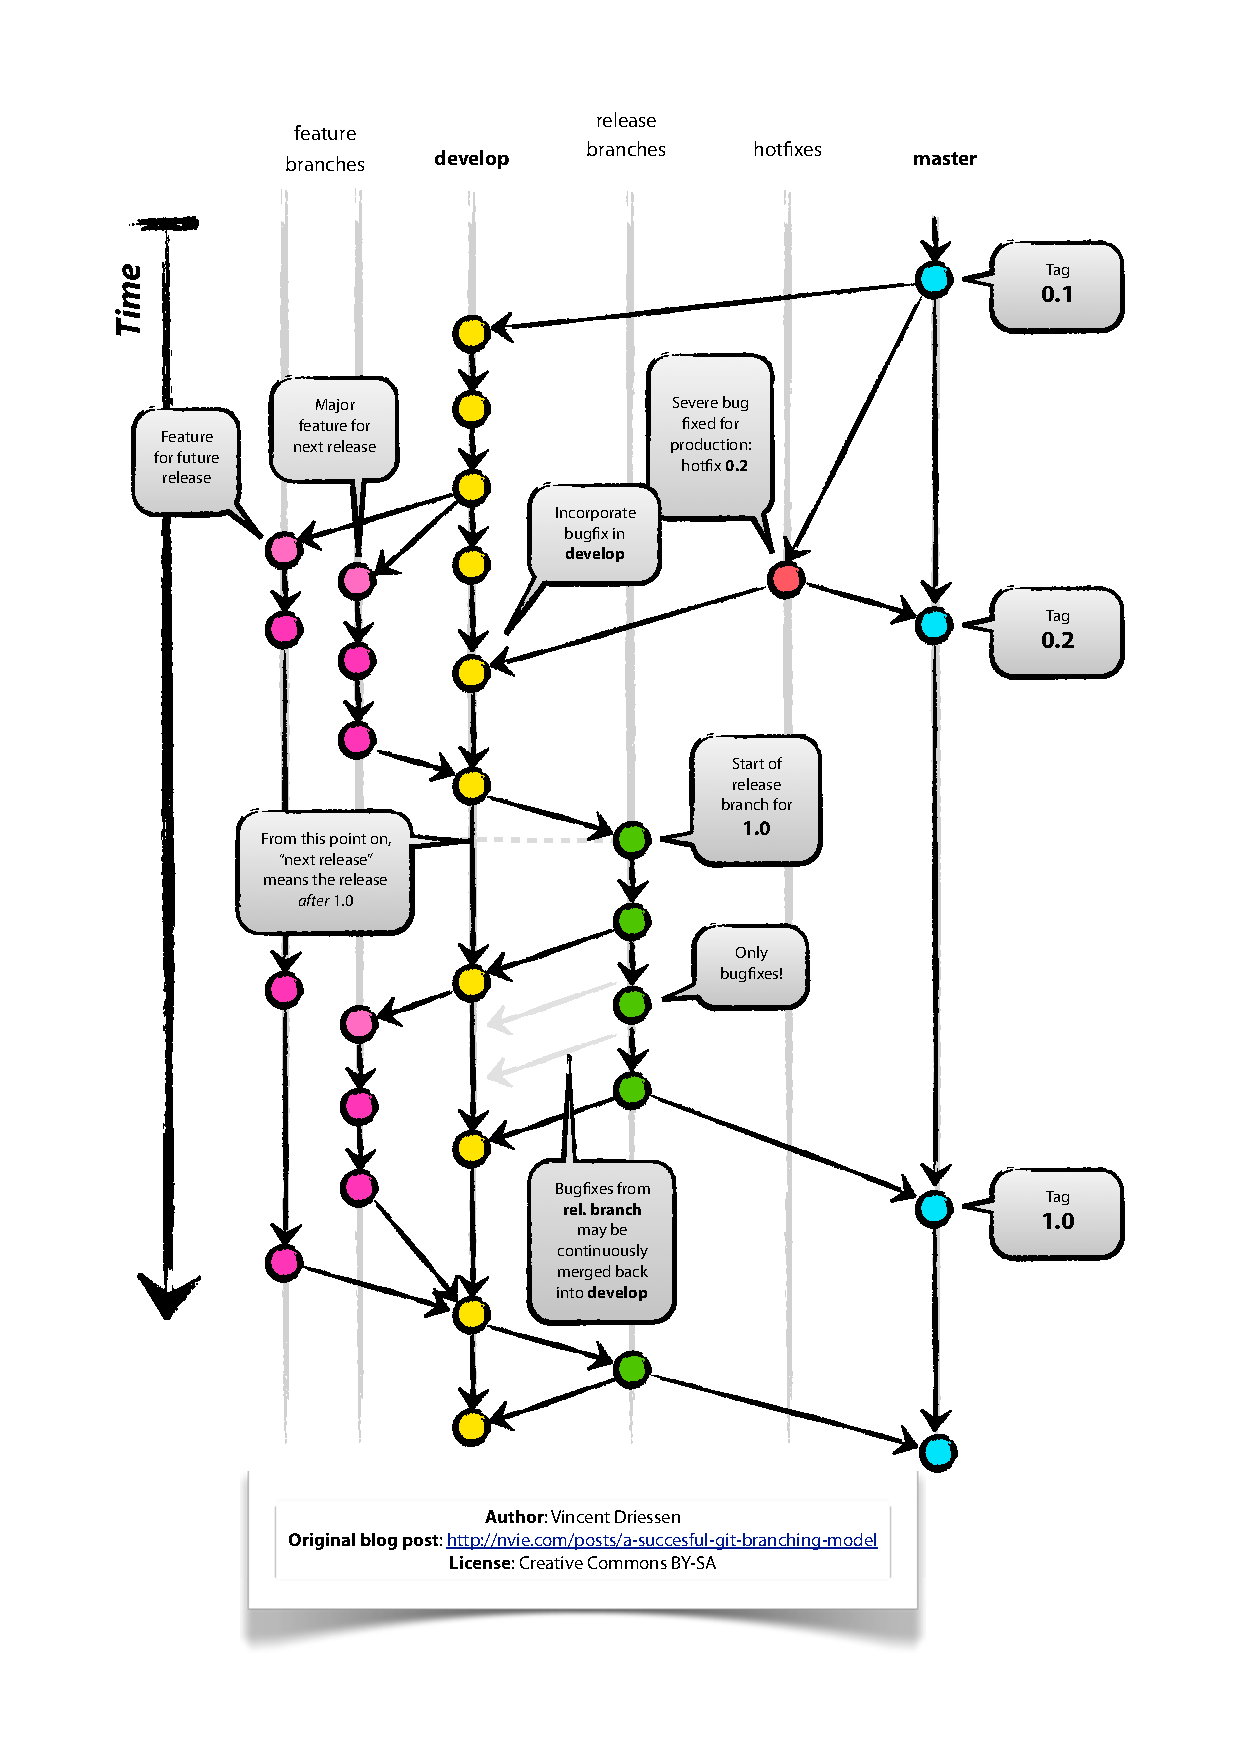
\includegraphics[width=0.5\textwidth]{img/Git-branching-model}
\end{center}
}

\fr{Lo stato dell'arte II} {
    \bl{Alcune considerazioni} {    
        \iz {
			\item Non lo useremo
            \iz{
                \item troppo complicato per i nostri scopi            
            }
            \item Comunque molto interessante perché racchiude tutti gli aspetti di un DVCS workflow
        }
    }

    \bl{I branch} {
		\iz {
			\item Sono il supporto fondamentale alle fasi del ciclo di vita del software 
			\item Ogni fase ha il proprio branch! 
			\item Branching e merging all'ordine del giorno!
		}
	}
}


\fr{Un modello più semplice} {
\begin{center}
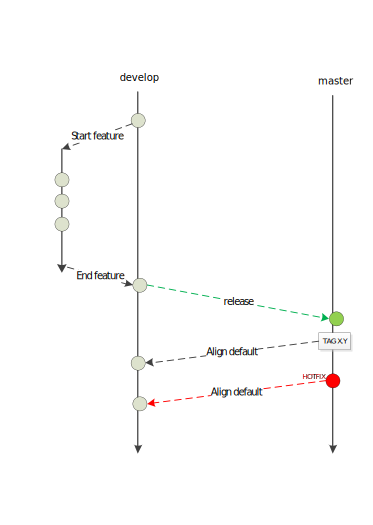
\includegraphics[width=0.5\textwidth]{img/visio-workflow-mercurial}
\end{center}
}

\fr{Rivediamo ruoli e compiti} {
\iz{
\item Sviluppatore: 
    \begin{enumerate}
        \item aprono un nuovo \textbf{feature branch} da \texttt{develop} ogni volta che cominciano lo sviluppo di nuova funzionalità
        \item le \textbf{feature} in realtà si aprono solo per funzionalità ``grandi'', altrimenti si lavora su \texttt{develop}
        \item effettuano commit regolari sul feature branch
        \item terminato lo sviluppo della funzionalità effettuano il merge della feature in \texttt{develop}
%         \item si occupano anche degli hotfix
    \end{enumerate}
\item Technical leader: 
    \begin{enumerate}
        \item supervisiona la qualità del codice prodotto
        \item è responsabile della qualità del codice che finisce sulla \texttt{develop} branch       
    \end{enumerate}

\item Release manager:
    \begin{enumerate}
        \item effettua i rilasci
        \item quando una nuova versione è pronta per il rilascio, effettua il merge della \texttt{develop} in \texttt{master} 
        \item effettua il tagging della release
    \end{enumerate}
}
}

\fr{Sulle feature branch} {
	Ha senso utilizzarle:
	\iz {
		\item per modifiche grandi o a rischio fallimento
		\begin{itemize}
		\item In particolare in termini di tempo richiesto per completare l'implementazione
		\end{itemize}
		\item Quando l'attività di analisi abbia già portato ad una classificazione accurata delle funzionalità
		\item Per separare e gestire meglio le attività di sviluppo in progetti articolati 
		\iz{
			\item chi fa cosa
			\item più sviluppatori impegnati sulla stessa funzionalità usano lo stessa branch            
		}
	}	
	In contesti articolati può quindi aiutare a tener traccia dello stato di avanzamento di determinate attività
}

\subsection{Comandi}

\fr{Inizializzazione del repository} {
\sizedcode{\tiny}{code/init.txt}
}

\begin{frame}[fragile, allowframebreaks]{Feature branch}
	\begin{center}
		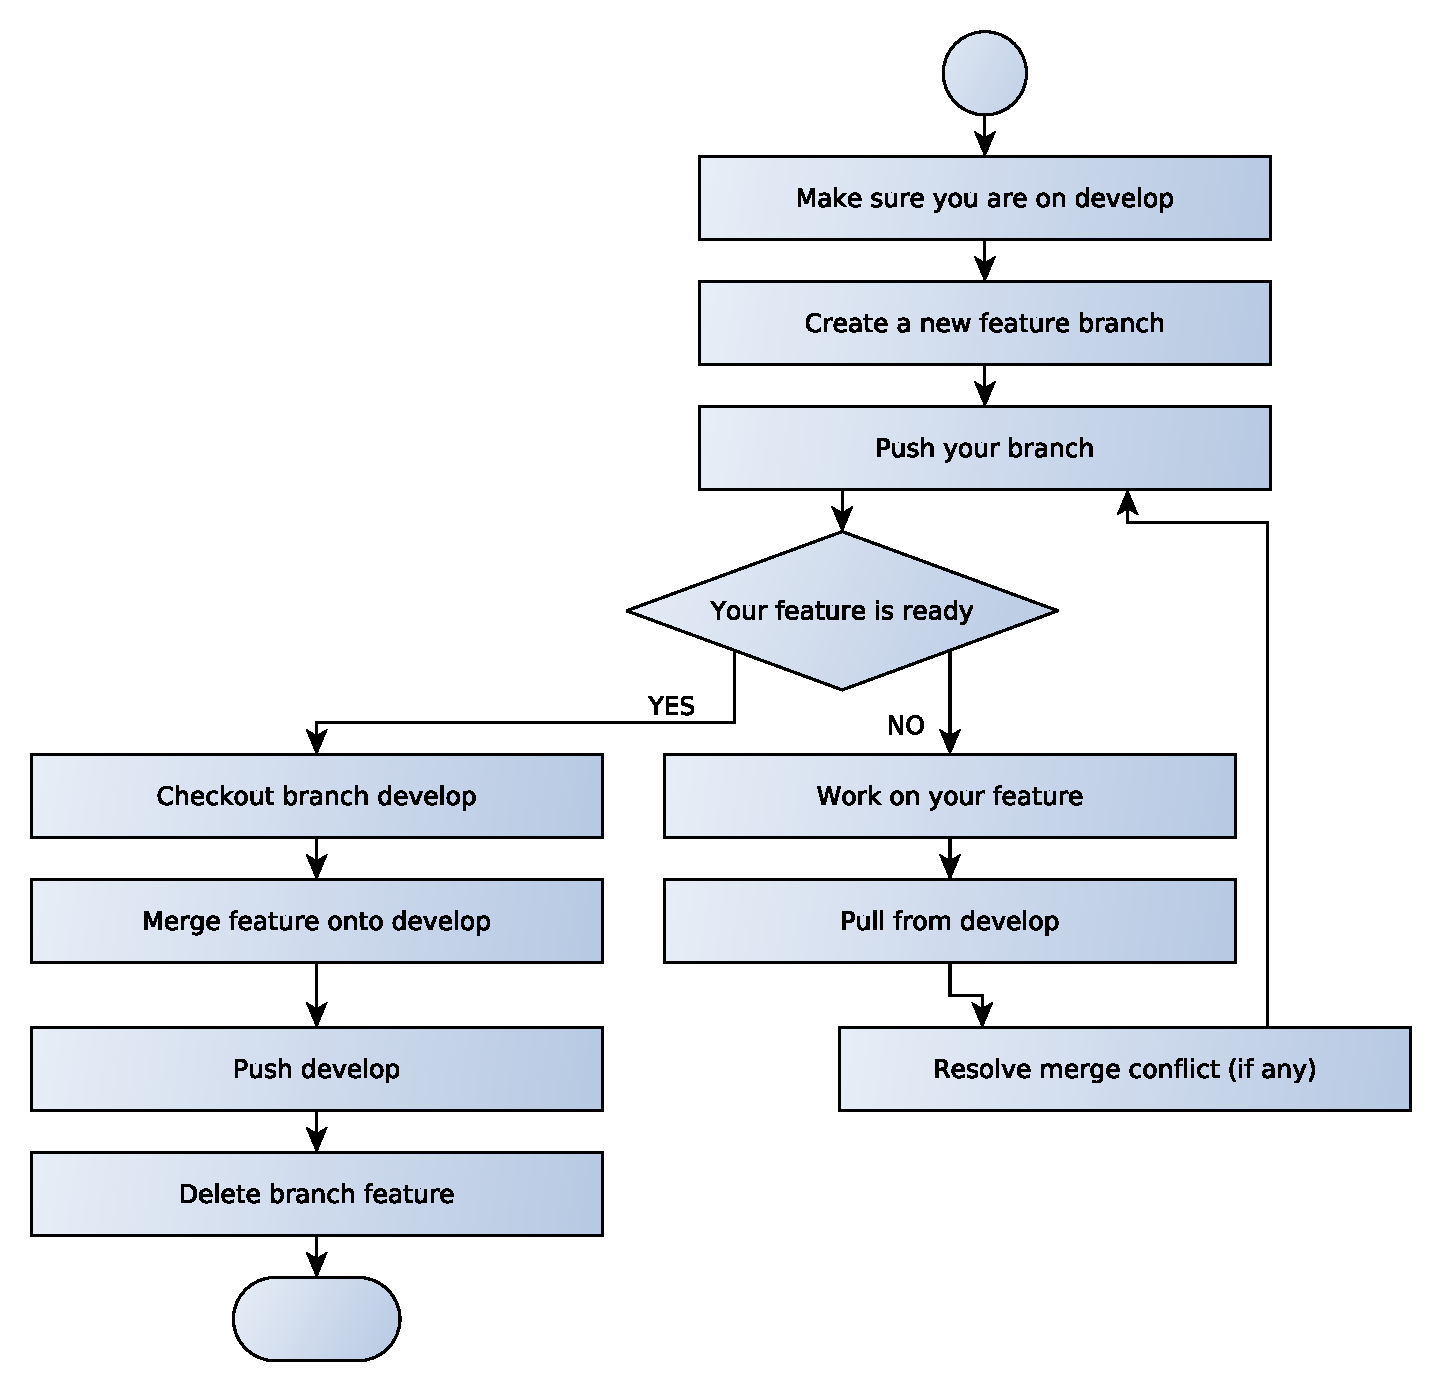
\includegraphics[height=.8\textheight]{img/feature}
	\end{center}
	\sizedcode{\tiny}{code/open-feature.txt}
\end{frame}

\begin{frame}[allowframebreaks]{Associazione di nomi simbolici ad un commit}
	\bl{In generale}{
		È necessario poter associare ad un commit della meta-informazione personalizzata. Ad esempio, per associare un certo commit ad una versione, in modo da poterla facilmente richiamare.
	}
	\bl{In Git}{
		\iz{
			\item \texttt{git tag -a MyTag -m "My tag information"}
			Associa al commit corrente il nome simbolico \texttt{MyTag} ed il messaggio aggiuntivo \texttt{My tag information}
			\begin{itemize}
				\item Non rimpiazza il commit message, ma lo integra
				\item È possibile invocare comandi come \texttt{git checkout MyTag} per tornare velocemente ad un tag precedente
			\end{itemize}
			\item \texttt{git push --tags}
			\begin{itemize}
				\item Fa \texttt{push} delle metaiformazioni aggiunte col comando \texttt{tag}
				\item La \texttt{push} ``normale'' non invia queste informazioni!
			\end{itemize}
		}
	}
\end{frame}



\fr{Fare una release} {
\sizedcode{\tiny}{code/do-release.txt}
}

\begin{frame}[allowframebreaks]{Il repo ufficiale del vostro progetto}
	\begin{block}{Workflow raccomandato}
		\begin{itemize}
			\item Qualcuno di voi agirà come ``repo maintainer''
			\item Creerà quindi il repository su BitBucket
			\item Gli altri membri del team faranno la \texttt{clone}
			\item Ciascuno lavorerà parallelamente sul proprio repository locale (working copy), condividendo tramite \texttt{push} e \texttt{pull} il proprio lavoro con gli altri
		\end{itemize}
	\end{block}
	\begin{block}{Workflow avanzato}
		Ottimo per progetti di grosse dimensioni e/o per team molto eterogenei, dove qualcuno deve assicurarsi della qualità del codice prodotto da altri.
		\begin{itemize}
			\item Il maintainer crea il repository, ed è l'unico col diritto di scrittura
			\item Gli altri membri del team hanno una fork a testa
			\item Ciascuno lavora su una working copy, facendo pull dal repository ``centrale'' e push sulla propria fork
			\item Quando una feature è completa, o si arriva ad un buon grado di sviluppo, si apre una \textbf{pull request}
			\item Il maintainer revisiona il codice, assegna eventuali modifiche, e quando è soddisfatto accetta la pull request facendo il merge del codice nel repository principale
		\end{itemize}
		Questo workflow è un overkill per il progetto di OOP
		\begin{itemize}
			\item Ma è possibile che vi chiederemo di lavorare così, se farete tesi o un tirocini relativi ad alcuni nostri software
		\end{itemize}
	\end{block}
\end{frame}

\fr{Best practice per la condivisione I} {
	Sviluppatore
	\iz{
		\item In generale, push regolare delle proprie modifiche su repo ufficiale (e pull regolare di quanto presente in remoto)
		\iz{
			\item Se il push riguarda il \texttt{develop} branch: le modifiche che condividete via push \textbf{devono compilare}!
		}
		\item Eseguire sempre un pull e update tutte le volte che cominciate a lavorare su qualche cosa in una certa branch 
		\item Per eventuali feature branch? Stesse regole di \texttt{develop}
	}
	Release manager
	\iz{
		\item Pull di \texttt{develop} prima di cominciare una release
		\item Push di \texttt{master} e \texttt{develop} al termine della release 
	}
}

\fr{Per approfondimenti...} {
A successful git branching model:\\
\url{http://nvie.com/posts/a-successful-git-branching-model/}
}
\end{document}

